\documentclass[11pt]{article}
\usepackage{a4, fullpage}
\usepackage{bibtopic}
\usepackage[small,compact]{titlesec}
\usepackage{float}
\usepackage{amssymb,amsmath}
\usepackage[T1]{fontenc}
\usepackage{graphicx}
\begin{document}
%\usepackage{multicol}
%\usepackage{multirow}
%\usepackage{listings}
%\usepackage{pdfpages}
%\usepackage{booktabs}

%\restylefloat{table}

%\setlength{\parskip}{0.3cm}
%\setlength{\parindent}{0cm}
%\setlength{\textheight}{10.7in} %used to be 10
%\setlength{\textwidth}{6.5in}
%\setlength{\parskip}{2pt}
%\addtolength{\oddsidemargin}{-.3in}
%\addtolength{\evensidemargin}{-.3in}
%\addtolength{\topmargin}{-.6in}
%\addtolength{\textwidth}{.6in}




%-------------------------------------------------------------------------------

%\title{\vspace{100px} BUSINESS PLAN \\ \vspace{100px} Shimla Gold Cider \vspace{100px}}
%\author{\vspace{50px}John Walker, Rutwik Shah, Sahil Jain, Alina Boghiu, Giovanni Charles, Łukasz Koprowski \vspace{50px}}

%Imperial College London, Department of Computing

%\date{\today}         % inserts today's date

%\maketitle           % generates the title from the data above

%\newpage

%\title{ \hspace{100px} SHIMLA GOLD CIDER BUSINESS PLAN}
%\maketitle

%\begin{table}[H]
%\begin{center}
%\begin{tabular}{| l | l |}
%\hline
%Date Stamp of this Document:     &  \today  \\ \hline
%Version of this Document:        &  V.0.2   \\ \hline
%Author/Editor of this Document:  & Adam Fiksen, \newline Alina Boghiu, \newline Giovanni Charles, \newline John Walker, \newline Rutwik %Shah, \newline Sahil Jain, \newline Lukaz Koprowski  \\
%\hline
%\end{tabular}
%\end{center}
%\end{table}


%-------------------------------------------------------------------------------

%-------------------------------------------------------------------------------
%    ALTERNATIVE TITLE PAGE
%-------------------------------------------------------------------------------



\begin{titlepage}
\newcommand{\HRule}{\rule{\linewidth}{0.5mm}}
\center
\textsc{\LARGE Imperial College London}  \\[1.5cm]
\textsc{\Large Department of Computing}  \\[0.5cm]
\textsc{\large Course 350: Management and Business for Computing Engineers} \\[0.5cm]

\HRule \\[0.3cm]
{\huge \bfseries Business Plan \\ \vspace{0.3cm}Shimla Gold Cider} \\[0.3cm]
\HRule \\[1.5cm]
\begin{minipage}{0.4\textwidth}

% author
\begin{flushleft} \large \emph{Authors:} \\
Alina     \textsc{Boghiu}    \\
Giovanni  \textsc{Charles}   \\
Adam      \textsc{Fiksen}    \\
Sahil     \textsc{Jain}      \\
\L ukasz  \textsc{Koprowski} \\
Rutwik    \textsc{Shah}      \\
John      \textsc{Walker}    \\
\end{flushleft}

% supervisors
\end{minipage}~
\begin{minipage}{0.4\textwidth}

\begin{flushright} \large \emph{Lecturer:} \\
Nick \textsc{Coutts}
\end{flushright}
\end{minipage}\\[4cm]

\end{titlepage}

%-------------------------------------------------------------------------------
\title{DISCLAIMER}
\maketitle

\noindent Although the authors has taken reasonable care to ensure that the information contained in this document is accurate, no other representation or warranty, express or implied, is or will be given by the authors or any of its agents. No responsibility is or will be accepted by the authors or any of its agents as to the accuracy or completeness of this document or the information or opinions contained herein.Recipients must make their own investigations and must satisfy themselves as to the condition and prospects of the authors and the accuracy and completeness of statements contained herein. \\

\noindent This business plan has been prepared by the authors and is being provided to a limited number of persons, at their request. This document is confidential and is only being made available to parties who agree to keep it confidential. Neither this business plan nor any part of it shall be copied, reproduced or distributed to others at any time without the prior written consent of the authors. By accepting this document the recipient is deemed to undertake and warrant to the authors that the recipient will keep it confidential and that the recipient shall return all copies of this document to the authors immediately upon request. \\

\noindent Any financial projections given in this plan are illustrative only. Because of the early stage nature of the authors' business, none of the projections given in this document should be taken as guaranteed to be attainable, nor should they be taken as implying any indication, assurance or guarantee that those assumptions are correct or exhaustive.
\vfill

\begin{table}[H]
\begin{center}
\begin{tabular}{| l l |}
\hline
Issued To:      &  Nick Coutts        \\
Company:        &  Shimla Gold Cider  \\
Submission date &  \today             \\
Copy Number:    &  1                  \\
\hline
\end{tabular}
\end{center}
\end{table}

\newpage
\tableofcontents

\newpage
%------------------------EXECUTIVE SUMMARY-------------------------------------%
\section{Executive Summary}
  \subsection{Overview}

  %A patented solution...
  %Vision to be...
Our mission is to bring a mid priced cider to the people of India. India has the second largest population in the world, and has an estimated market size of 500 million alcohol consumers [better estimate]. At the moment, there is one provider of cider in India, and we would like the change that. \\

\noindent We want to be a brewery. We will brew our own cider in the state of Himachal Pradesh, which is the source of the majority of the apples in India. Along with producing cider, we will sponsor other exclusive bars and clubs. \\

\noindent Operating in India which is well known for its corruption, we want to practice ethical development. eg corrupt free, no bribes, no blood cider forced labor fairtrade \\

\noindent We hope to gain popularity in major establishments, in Delhi and Mumbai through the open minded youth and bar owners. \\

\noindent Our cider will become a desired commodity through exclusivity and we will be able to research our market further at this point with minimal risk. \\

\noindent We will adapt and pick up popularity and scale up to make it available to the public.
  %Consumer and regulatory pressure...
  %Has clear competitve advantages...
  %Has unsurpassed technology and has sales through...

  \subsection{Market Drivers}
Marketing is all about creating value for the customer and striving to meet and then exceed customer expectations.\\

\noindent Market driver or drivers are considered at the time envisaging and establishing value of a product/service that's to be marketed. \\

\noindent These drivers are primarily trends that cause an existing or new market to develop. In our case, There is a large market for alcohol in India, who are eager to try out new things, which can be seen by the successes of these microbreweries. As India continues to grow to become a bigger powerhouse in the world, it will attract more foreigners, which means that people who already know about cider and like it will increase in the country. This increasing market size makes us believe that cider will become increasingly popular in India once introduced properly. \\

\noindent The four elements of segmentation especially psychographic and behavioral segmentation are key tools in determining these trends. \\

\noindent So at the end of the day, you'll be able to then understand how and why the market is changing, causes of the change and eventually looking out the window that will show how new opportunities are developed. \\
  %Market drivers....

  \subsection{Business Proposition}
  %Meets increasing demands...

  \subsubsection{Business Requirements}

In order to reach our ultimate goal of becoming a major supplier of 
cider in India, we have formulated some requirements in order of priority: 
  
  \begin{table}[H]
  \begin{center}
  \begin{tabular}{| p{7cm} | p{7cm} | p{7cm} | p{7cm} | p{7cm}}
  \hline
  Abstract & Ambition & Impacts & Meter & Scale\\
  Likeability & A good and popular product is the foundation of our company.
Without a following we will not be able to turn the profit we require to survive
 & A likeable brand/product will generate high demand and revenue draw
investment. However this will come at a monetary cost & Taste & Market testing feedback\\
  &&&Brand image & brand reach through number of distributors, exposure through
social media statistics, successful promotion events\\
  Economical & Once our business is showing potential we can streamline the
manufacturing process in order to generate a profit and in turn growth & reduced costs and increased profits. This comes at a cost of the research and development effort& Waste & mass of raw materials - final product mass \\ 
  &&&Meeting demand & aim for "one bottle left on the shelf",
under/oversupply\\
  &&&Production cost & cost of production per bottle - 20rps\\
  Ethical & Though it may be hard to achieve at first, we must attempt to be
ethical out of principle. These practices may also result in respect in the
industry and our consumers & May result in reduced profits but could also encourage
productivity and efficiency & fairtrade & \% of profits seen by downstream
suppliers\\
  &&&Reducing waste as above &
  \end{tabular}
  \end{center}
  \end{table}

  \subsubsection{Timeline}
After marketing planning and researching the development process we have decided upon a 7 month timeline for our business plan, encapsulating everything from setting up to starting the distribution of our product. The latter constitutes the end point of our business plan and a stable milestone after which the company can be considered self sustainable. Following are the three main stages of our timeline.

  \begin{enumerate}
  \item Licensing and building - 1 month
    \begin{itemize}
    \item Register company
    \item Obtain brewing license
    \item Rent space
    \item Setup utilities: contracts and infrastructure
    \end{itemize}

  \item Staff recruitment - 1 month
    \begin{itemize}
    \item Advertise job availability
    \item Process applications and interview applicants
    \item Start the training process as soon as we hire a qualified individual (brew master)
    \item Order equipment: it should have time to arrive by the time training is finished
    \end{itemize}

  \item Market research - 5 months\\
  This phaze constitutes of daily iterations of the following sequence:
    \begin{itemize}
    \item Produce small quantities of a recipe variation (with an offset of 20 days for fermenting)
    \item The professional taster tests the product and offers feedback
    \item The team and brewmaster distribute to locals and collect feedback
    \item The team and brewmaster reach out to distributors with samples of the product we are perfecting
    \item File for a patent on our final recipe.
    \end{itemize}
  \noindent After 5 months the recipe should be perfected and contracts with distributors signed. The only change that must be made at this point is upping the production scale to meet the request. The equipment will be in place for this.
  \end{enumerate}

  \subsection{Financial Summary and Investment Proposition}
     For our Initial investment we require at current conversion rate an initial amount of Rs. 11,00,000 due to the large number of us participating in this project we do believe this amount is small enough for us to raise this through friends and family. We do believe starting a small business through this will provide us with flexibility to create a business model without having to answer to anyone. If run correctly, it will give the us the opportunity to earn more, with more freedom and independence.\\
     The First 9 months we intend to set up our brewery and perfect our product. This also provides time to market our product and spread word of its release. After this we intend to release the product into a few major cities through distributors

\newpage
%------------------------------------------------------------------------------%
%------------------------MARKET OPPORTUNITY------------------------------------%
\section{Market Opportunity}
  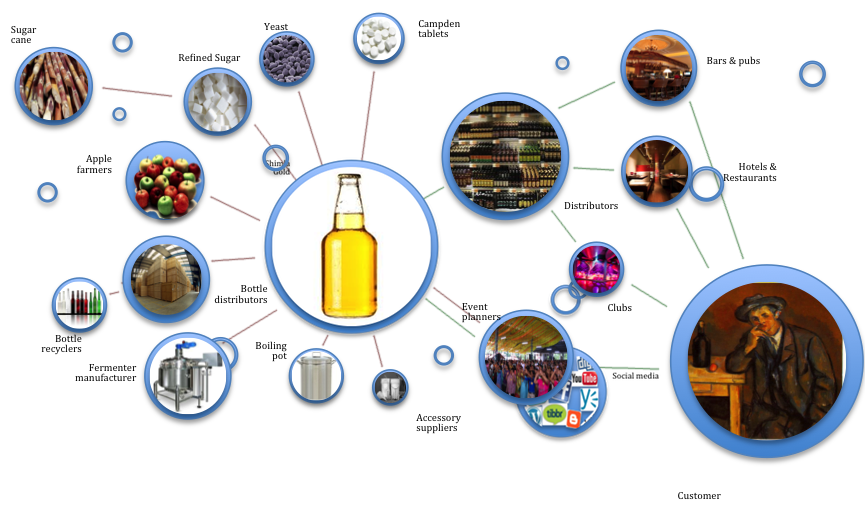
\includegraphics[angle=90,width=\textwidth,height=\textheight,keepaspectratio]{./supplychain.png}
  \subsection{The Opportunity for Shimla Gold Cider}

India is an increasingly growing economy where the common man is getting richer by the day. As people are getting richer, they are getting more money to spend on pleasure. Due to this increase in flux of money, people are willing to pay more than they used to on going to bar/pubs, which has become a common night out for the population. \\

\noindent As the demand for alcohol increases, we have found an untapped market. Currently, there is only one manufacturer of cider in India, which itself is becoming increasingly popular. In 2006 in the United Kingdom, 600 million liters of cider are produced annually. Beer is very popular in India, and it has been growing steadily at a rate of 10\%-17\% over the past 10 years. Around 170 million cases (12 bottles) of beer were produced in the financial year 2008-2009. \\

\noindent These figures indicate that there can potentially be a large market for cider in India, and we believe that Shimla Gold Cider can make it big in India if it is produced and marketed well. \\

\noindent As we can see, there is a large market for alcohol in India, who are eager to try out new things, which can be seen by the successes of these microbreweries. As India continues to grow to become a bigger powerhouse in the world, it will attract more foreigners, which means that people who already know about cider and like it will increase in the country. This increasing market size makes us believe that cider will become increasingly popular in India once introduced properly.
  %Addressable market of...

  \subsection{Market Segments}
 Although we are going to be selling our product to alcohol distributors,
we want to make it appealing to the younger population of India. We are aiming
for this product to be sold in the bigger cities of India, such as New Delhi,
Mumbai and Bangalore. We believe that these are the types of cities were we can
obtain maximum profit.
Along with this young crowd, we are aiming the cider to tourists and foreigners
living in India. As these people know what cider is, and quite a few of them
like cider as well, we think that this provides us with a greater market
potential.
It is widely regarded in the Western world that women prefer cider to beer due
to the sweeter taste. Currently in India, there is no equivalent to beer for
women, so we believe that women would be a large proportion of our customers.

\newpage
%------------------------------------------------------------------------------%
%------------------------PRODUCT PROPOSITION-----------------------------------%
\section{Shimla Gold Cider Product Proposition}
%Has superior technology in....
\subsection{Shimla Gold Cider's Unique Proposition}

We aim to provide our cider efficiently and cost effectively with our custom
brewing system. By purchasing our equipment in parts we are able to ensure that
they are good quality, we are agile enough to expand and we are not paying for
the convenience of a complete package.

Our modern approach to advertisement, exploiting social media and events, should 
gain far reaching and focused exposure. We expect Shimla Gold to become a
household name, helped by the fact that it will naturally be set apart from its
competitors in the beer industry. 

After our testing iterations we will 
have a Shimla Gold will be one of the few ciders on the market, not to mention 
tuned to the tastes of the Indian public. This will be desirable product which 
should command a strong market power.

  \begin{enumerate}
    \item Ingredients for dry, sparkling cider, 10.5\% abv (per gallon of cider)
	  \begin{itemize}
	   \item Apples - 7kg
	   \item Yeast (English Cider) - 2g
	   \item Campden tablets - 1
       \end{itemize}
	\item Ingredients for sweet, sparkling cider,10.5\% abv (per gallon of cider)
	  \begin{itemize}
	  \item Apples - 7kg
	  \item Yeast (Sweet Mead) - 2g
	  \item Sugar - 250g
	  \item Campden tablets - 1
	  \end{itemize}
	\end{enumerate}

  \newpage
  \subsection{Business Model}
  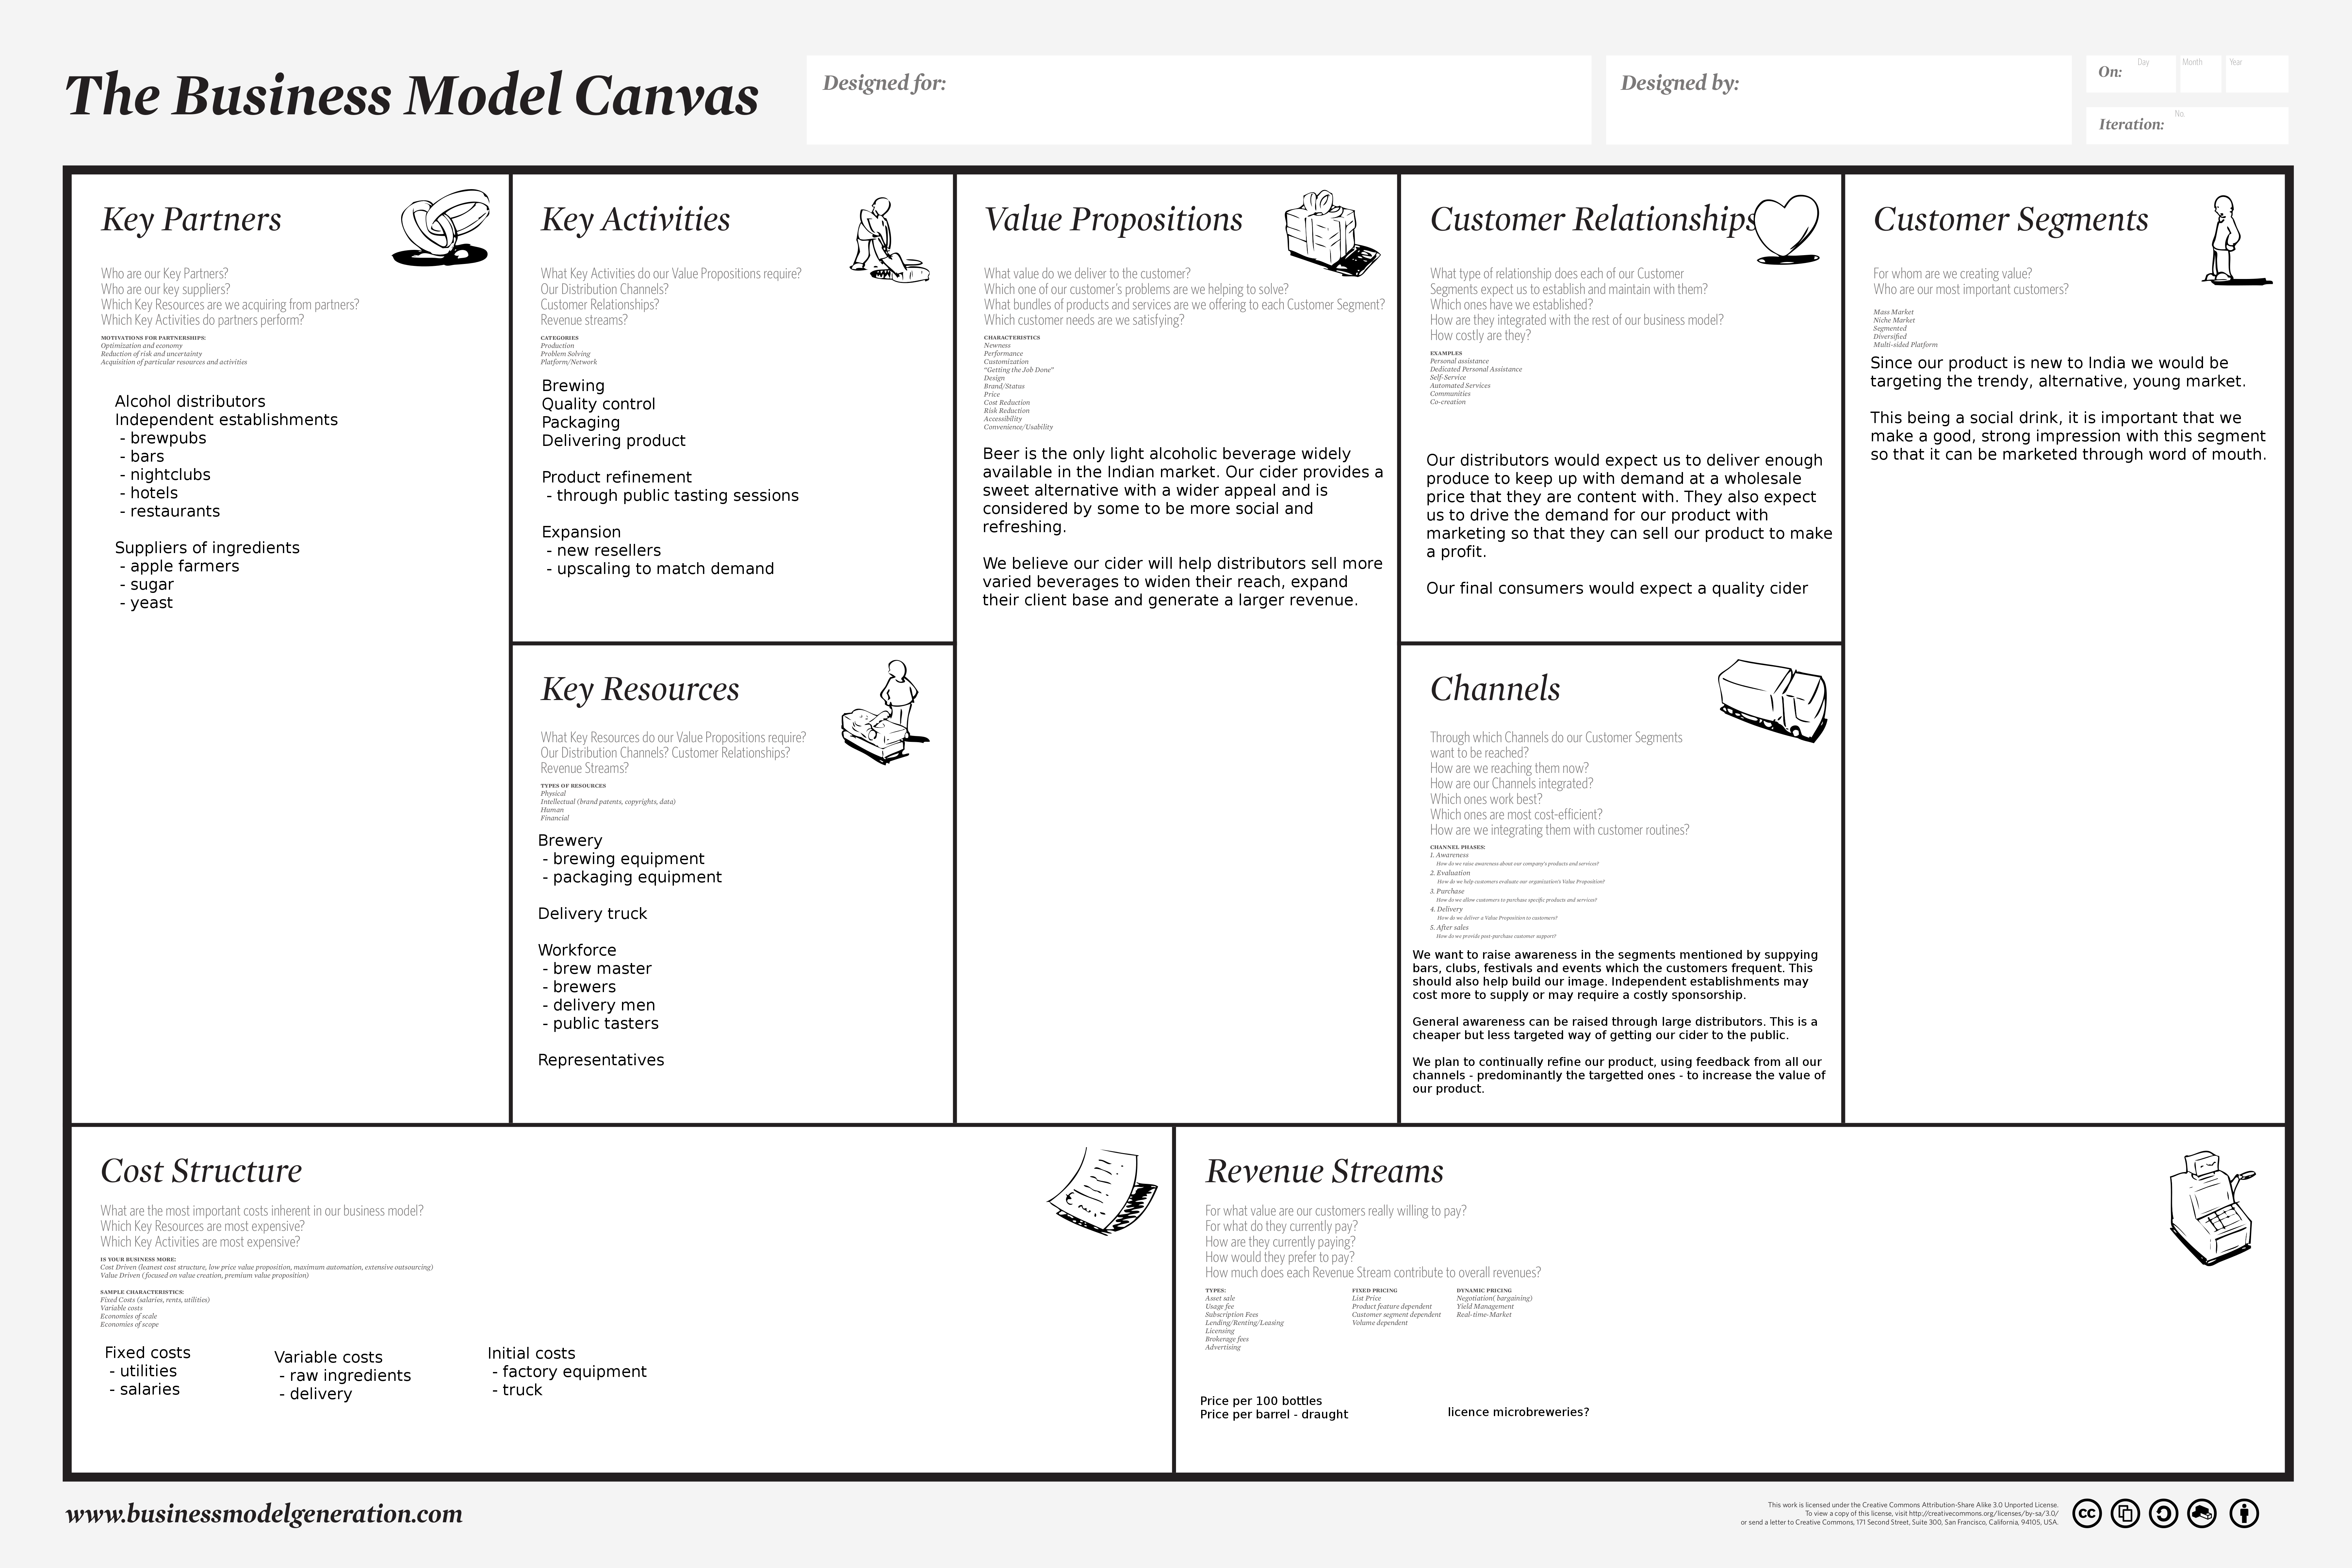
\includegraphics[angle=90,width=\textwidth,height=\textheight,keepaspectratio]{./business_model_canvas_poster.png}
   %Established production, sales & marketing, distibution model...

\newpage
%------------------------------------------------------------------------------%
%------------------------TARGET MARKET-----------------------------------------%
\section{Target Market}
  \subsection{Market Context}
  %Global vision well defined market segments and territories...
		Although we are going to be selling our product to alcohol distributors,
		we want to make it appealing to the younger population of India. We are aiming
		for this product to be sold in the bigger cities of India, such as New Delhi,
		Mumbai and Bangalore. We believe that these are the types of cities were we can
		obtain maximum profit.
  \subsection{Market Size and Characteristics}
  %This equates to a global revenue opportunity of???
		Calculating an estimate of the total alcohol consumers in India (figures are rounded to make calculations simple):
		\begin{center}
			\begin{tabular}{ | c | c | }
				Population of India & 1400000000 \\
				Life Expectency & 70 \\
				Assume that there are an equal number of people in each age bracket & \\
				Every 10 year age bracket & 200000000 \\
				People under 25 are illegal to drink & \\
				People who can consume alcohol & 900000000 \\
				Assume that the male to female ratio is 1:1 & \\
				Total Male & 450000000 \\
				Total Female & 450000000 \\
				Assume 75% of men drink alcohol & 337500000 \\
				Assume 40% of women drink alcohol & 180000000 \\
				Total alcohol consumers & 517500000 \\
			\end{tabular}
		\end{center}

		This number is not an accurate representation of our potential market,
		because not every one could afford to buy our cider. Assuming that
		we can target our target to the top 10% of this market, we get a potential
		market size of around 50 million people.

  %Diagram yearly market potential
  \subsection{Market Validation}
  %Has met all technical norms

\newpage
%------------------------------------------------------------------------------%
%------------------------COMPETITION-------------------------------------------%
\section{Competition}
%Limited number of direct competitors
	\subsection{Current Competitors}
There is only one manufacturer of cider in India at the moment. Green Valley Cider produces Tempest Cider, which is a 8\% cider, in the state of Himachal Pradesh, where they own several acres of apple orchards. Tempest cider are sold at Rs 60/- per 330ml bottles, and for Rs 105/- per quart. The most recent figures of Tempest Cider sales indicate that in 2007, around 50,000 cases of 12 bottles each were being sold annually. Currently, Tempest Cider is not available in the big cities of India such as New Delhi and Mumbai. \\

\noindent Some exclusive alcohol stores in India sell imported ciders, but these are very rare. The price of these imported ciders is very high as well, due to the high 150\% alcohol import tax.

  \subsection{Competitive Advantage}
  %Competitve advantage in technology

\newpage
%------------------------------------------------------------------------------%
%------------------------MARKET DEVELOPMENT PLAN-------------------------------%
\section{Market Development Plan}
  \subsection{Sales Process}
  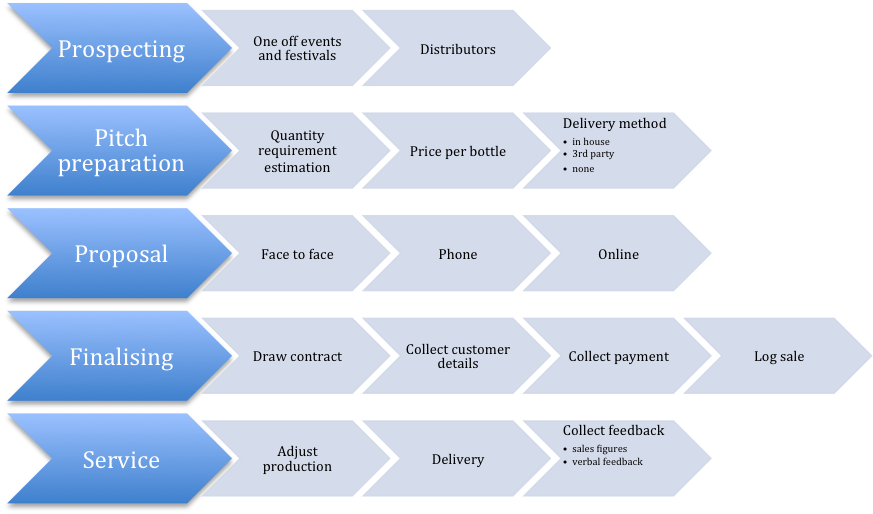
\includegraphics[width=\textwidth,keepaspectratio]{./process.png}
  %Good relationship with strong distributor...

As we are setting up a small brewery, reaching millions of potential of customers across several cities will be very difficult and more than that expensive. Hence we decided to use a distributor, namely, Elan Distributors Inc. The distributor buys a majority of our product and sells it to several pubs and lounges around the country at a slight mark-up compared to what we sold it to them at. Then based on demand of the product, the distributor, will provide notice for how much they want to purchase. Further if this product does well the distributor may demand exclusive rights to selling our product which would earn us additional revenue.

  \subsection{Target Customers}
  %Larger customers as targets
  Our target customers are young aspiring customers from middle and upper class households.
  It is estimated that by 2030 their number will grow by 130 millions.
  Looking at the growth of income and changes to the policies beer will become affordable to a growing number of people in India.
  Consumption is supposed to rise 12.5 times due to these factors.
  This creates a perfect growth opportunity and makes this group of customers most valuable.

  \subsection{Current Key Customers}
  %Large current customers
  Our current key customers is educated and aspiring youth in larger cities.
  As we know from conducted research this is a group that is most influential and has the biggest potential.
  Western influence already increases popularity beer, cider and low alcoholic beverages.
  A trend that is not likely to go away.
  We also start by distributing our product among young professionals because they are the ones who drive trends and set new standards.

  \subsection{Marketing, PR and Communications}
  %Marketing and market awareness crucial..
We aim at advertising through college fairs this comes at a cost of Rs. 10,000 in a majority of colleges. For this small number there are several benefits:
\begin{enumerate}
\item Conduct contests of skill and award prizes to the public to generate interest.
\item Have full rights for on-site branding across the stands.
\item Have its CEO / nominee present the trophies of certain
\item Be entitled to the free use of lawns to interact with students.
\item Arrange for live entertainment before or after the event.
\item Promote and your brand via mailers/press.
\item Have access to the College's student data which consists of thousands of potential customers who represent some of the most clients we are targeting in India.
\item Have promotion on the website with links to the lounges webpage.
\end{enumerate}

We would also like to use as much social media as possible to create brand awareness. This can be done through use of Facebook, Twitter and such websites where we can encourage sharing and liking  of pictures with small prizes.//

We would sponsor student parties which will significantly increase the initial consumption of our product and increase awareness.

\newpage
%------------------------------------------------------------------------------%
%------------------------INTELLECTUAL PROPERTY (IP) ASSETS---------------------%
\section{Intellectual Property (IP) Assets}
  \subsection{Shimla Gold Cider Solution}
    \subsubsection{Patents}
    Cider is an age old product and we are using already existing machinery to
    produce it therefore the number of patents we can take out is limited we will
    be looking to take out the following patents.
    \begin{itemize}
    	\item Recipe \\
We will be looking to take out a patent on the recipe for our cider this means the recipe has to meet 4 criteria:
 	      \begin{itemize}
		    \item It has to be patentable subject matter, a recipe is a new 'composition of matter' therefore it is patentable.
		    \item It has to be useful. Virtually everything is considered useful.
		    \item Is it novel and non-obvious. This might be harder to prove as cider is such an age old recipe but we could argue that our new use of Indian Shimla apples is novel
	      \end{itemize}
If we fail to obtain a patent on our recipe we would have to resort to simply keeping the recipe a secret this has worked for many companies in the past. Our recipe will be a unique blend of various types of apple and flavour brewed in a particular way using particular equipment it will be very hard to reproduce and by the time any one had we would hopefully have a large market share making it harder for competitors.
	\item Name \\
    We will be looking to trademark the name of Shimla Gold Cider.
	\item Logo \\
    We will also be looking to patent the logo for Shimla Gold Cider.
    \end{itemize}
Obtaining these patents will cost around £220.\textbf{[this belongs in the finaince secion]}

    \subsubsection{Know-How}
    %Internation experts choose to work with X

  \subsection{Future IP Developments}
  %Future applications plannes along with IP Protection...
Although not as pressing as our cider, we will also be looking to to take of patents soon after we start production of the the cider for our subsidiary apple juice product this will include the recipe, name and logo. Obtaining these patents will cost a further £220. \textbf{[this belongs in the finaince secion]}

\newpage
%------------------------------------------------------------------------------%
%------------------------BUSINESS GROWTH AND RESOURCE PLANS--------------------%
\section{Business Growth and Resource Plans}
In order to setup a stable and long lasting infrastructure for our business we must take into consideration all the stages and requirements of production. Researching our cider recipe constituted the guideline and starting point of a coherent development plan.

  \subsection{Current Structure and Resources}
  %Early phase centred on technology development
The favorable aspects of our current situation is our team of young, dynamic individuals, excited about implementing a good business idea. We are fast learners, on our way to obtaining university degrees, with a great tolerance to change and fully capable of taking on unforeseen obstacles without being overwhelmed by minor defeats. We believe a positive, persistent and energetic attitude towards implementing any business will yield a positive result and a great learning experience.

  \subsection{Staff Recruitment}
%The average cost of hiring for the skilled workers is about 1,00,000 a year we would require :
% Keep all the cost and finance information in one well defined section
  \begin{enumerate}
  \item Qualified Brewmaster \\
He has to have previous experience with brewing various types of cider and would probably have to be recruited from a country with cider making traditions (France, England). He would serve as our cider making expert, being able to swiftly operate the equipment and professionally asses the quality of our cider. He must also supervise the general staff activity and behaviour.

  \item Microbiologist \\
He would serve as an assistant brewmaster, and would be responsible for conducting cider quality control tests, and performing microbiological analysis. He must also verify all the ingredients including the apples, sugar, yeast and water.
It is important to ensure a good quality especially considering the novelty of our product for this market.

  \item Unqualified labour \\
Our microbrewery requires manual labour as described below. These employees must work with the equipment we provide, attend to washing and maintaining it with responsibility. Therefore brief training must be considered as a cost. \\
  2 workers in charge of apple receival, washing and sorting
  2 workers in charge of apple grating
  2 workers in charge of apple pressing
  1 worker in charge of general cleaning of the area

  \item Security guard \\
On top of general surveillence, he is in charge of verifying employee ids and greeting visitors.
  \end{enumerate}

% same here, all cost information in one place
% Further as required we will require a security guard which will cost about Rs. 50,000 a year.

  \subsection{Facilities}
    \subsubsection{Space requirements}
When deciding upon our homebase we considered firstly our situation as a new business, with no existing assets or experience, as well as the small scale of our production line. We have also based our decisions around the brewing process, the stages of which are described in the figure below\\

\begin{figure}[h!]
\centering
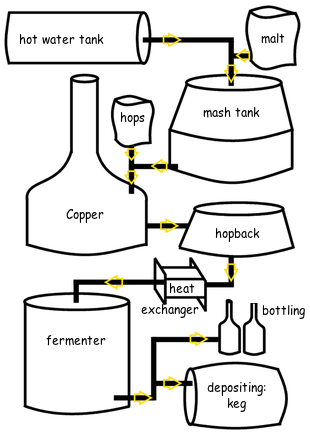
\includegraphics[scale=5]{brewing.png}
\end{figure}

\noindent We are aiming to brew \emph{15 gallons per day}. Whilst we will start off by brewing small quantities in order to perfect the recipe, we must setup the scale which we need for efficient and profitable distribution. We have already identified the ingredients quantity requirements per gallon when researching the recipes we will use and have explained how these might change. Using this information, these are the room size and functionality requirements we identified: \\

  \begin{enumerate}
  \item Ingredients handling room \\
  This room must be easily accessible by our providers and large enough to store a week's worth of ingredients including:
    \begin{itemize}
    \item 1500L refrigerator to store 630Kg of apples
    \item 23kg of sugar
    \item yeast, campden tablets
    \end{itemize}
  The room must have a constant supply of water for washing apples and equipment. \\
  The room will operate a weekly pipeline of ingredients storage, however spare space must be available for unforeseen situations.\\
  The room size must also allow washing, grating and pressing of apples which implies equipment and staff as detailed in the following sections.

  \item Brewing room \\
  This room must accommodate the two brewing systems for dry and sweet cider: approximately $2m^3$ each. It must also be able to fit a desk and file cabinet for general office equipment.
  \item Fermenting room \\
  This room will operate a daily pipeline and must be able to accommodate a weeks worth of produce: $4m^3$. It must maintain a constant temperature of approximately $22^\circ$C for fermentation. We have decided upon this as a good trade-off between quality and speed which are inversely proportional: a lower fermenting temperature yields higher quality but requires more time. However this is a specific decision the brewing master must make daily.

  \item Bottling and storage room \\
  The bottling room must accomodate enough space to hold our 2 kegs/day as well as the bottles the cider goes into -- assuming we produce about 20 gallons a day in full production, that requires about 230 bottles a day. The space required for this is roughly $1m^3$. We then need to take into account how regularly we will receive pickups from distributors --about one week. This results in a room of at least $7m^3$ for storage, plus space to actually perform the bottling. \\
The bottling work will be done with the use of `bottling wands' which allow a consistent amount of cider to be poured per bottle, as well as keeping the cider from oxygenating. For our fizzy ciders, we will introduce about 3.3g of sugar per bottle to allow secondary fermentation to occur. These filled bottles are then handed off to a capper, who will place the caps on each bottle, use the bottle capper to tighten the caps and place them in to boxes for storage.

  \item Maintenance room\\
  This should be a small room for storing cleaning equipment. It should have access or be attached to a staff restroom.
  \end{enumerate}

    \subsubsection{Equipment requirements}
    \begin{enumerate}
    \item Production equipment
      \begin{itemize}
      \item Apple wash tub
      \item Apple crushing device
      \item Hand cracked cider press: small
      \item Mash tank: 15 gallon
      \item Sparge tank: 15 gallon
      \item Boil Kettle with a false bottom and a siphoning tube
      \item Chill wizzard with a cold water hoze and oxygen pump
      \item Fermenting tank with blow up valves for speedup: 15 gallon
      \item Propane burner
      \end{itemize}

    \item Storage equipment
      \begin{itemize}
      \item 1500L refrigerator for apple storage
      \item freezer for excess and spare apple woat
      \item Fermenting tanks: as mentioned above, in order to host the weekly pipeline, we require 7 15 gallon tanks and spares.
      \item bottles: we are aiming for a production line of 210 bottles daily therefore our weekly requirements is of approximately 1300 bottles including spares
      \item boxes and labels
      \item shelves or containers ingredients (which come in their own boxes)
      \end{itemize}

    \item General maintenance equipment
      \begin{itemize}
      \item air conditioning system: for the fermentation process
      \item security alarm ans surveillance system
      \item fire detection system
      \item water filtering system
      \item cleaning equipment:
        \begin{itemize}
        \item chemical substances (pbw socution, idophor)
        \item cleaning substances (soap, bleach)
        \item blue roll, toilet roll, cloths
        \item bags, bin bags
        \item hozes, gloves, brooms, mops, buckets
        \end{itemize}
      \item office equipment:
        \begin{itemize}
        \item paper and pens
        \item company stamp, files, plastic sleeves, paper punch, envelopes, stapler and staples, disposable cups, bin
        \item employee register book, visitor register book
        \item company landline telephone
        \item company laptop
        \item tea, coffee, water
        \item first aid kit
        \end{itemize}
      \end{itemize}
    \end{enumerate}
\newpage
%------------------------------------------------------------------------------%
%------------------------FINANCIAL PLAN AND FUNDING ASSUMPTIONS----------------%
\section{Financial Plan and Funding Assumptions}
  \subsection{Financial History}
	\subsection{Pricing}
	We aim at pricing our cider at about Rs.80 which falls in line with most other mid range beer prices. Hence allowing people to try this cider as an alternative to beer. For a majority of indians it  will be viewed in the same lines. Though this is slightly more expensive than other local beers like Kingfisher available at roughly between Rs 40 - Rs.50 , it will provide a level of slight level exclusivity much desired by the growing youth in India.

	\begin{figure}[h!]
	\caption{Beer Prices India}
	\centering
	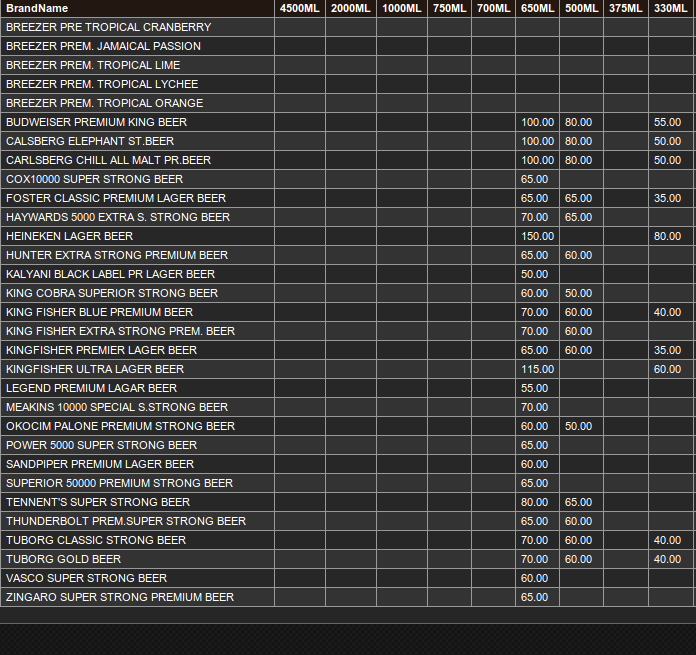
\includegraphics[width=\textwidth]{beerprices.png}
	\end{figure}
  \subsection{Financial Projections}
Initially our main source of revenue would stem from sale of products in the short run. Once we establish our brand through advertising and sale through different pubs and restaurants, we would like to further increase volume of sales and production and increase revenue through sponsors. In the long run we would like to further increase our product range including different flavours of ciders and gradually streamline our distribution process. This will all result in economies of scale hence reducing cost and added the product range will increase volume of sales. We have shown a projection for our product for the next few years.
	\begin{figure}[h!]
	\caption{Financial Projections \newline Note: it should be noted however that for the first 9 months there are a lot of initial cost for getting equipment with no sales for the first 3 quarters \newline the exact figures have been attached in the Annex 3}
	\centering
	%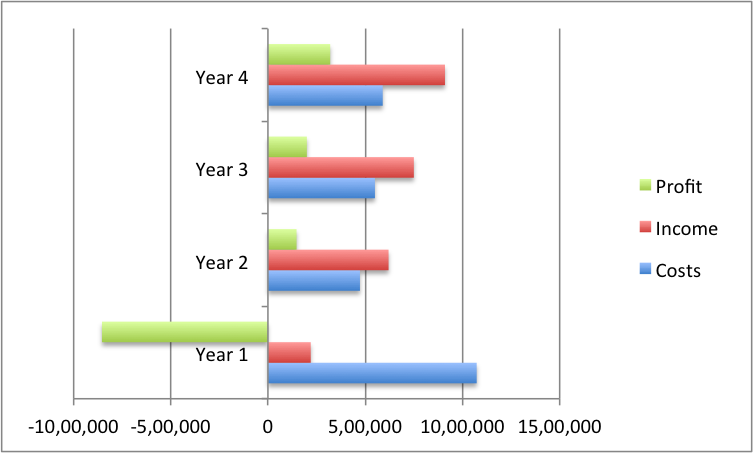
\includegraphics[width=\textwidth]{financialProjections.png}
	\end{figure}


  \subsection{Use of Funds}
The initial Rs, 11,00,000 which we aim to raise throughout friends and family has been listed as follows.
Following this period all cost will be easily met using the revenue earned from the sale of our product. //
The exact breakdowns of cost have been further provided

	\begin{figure}[h!]
	\caption{First Year Month Wise Cost \newline Note: the exact figures have been attached in the Annex 3}
	\centering
	%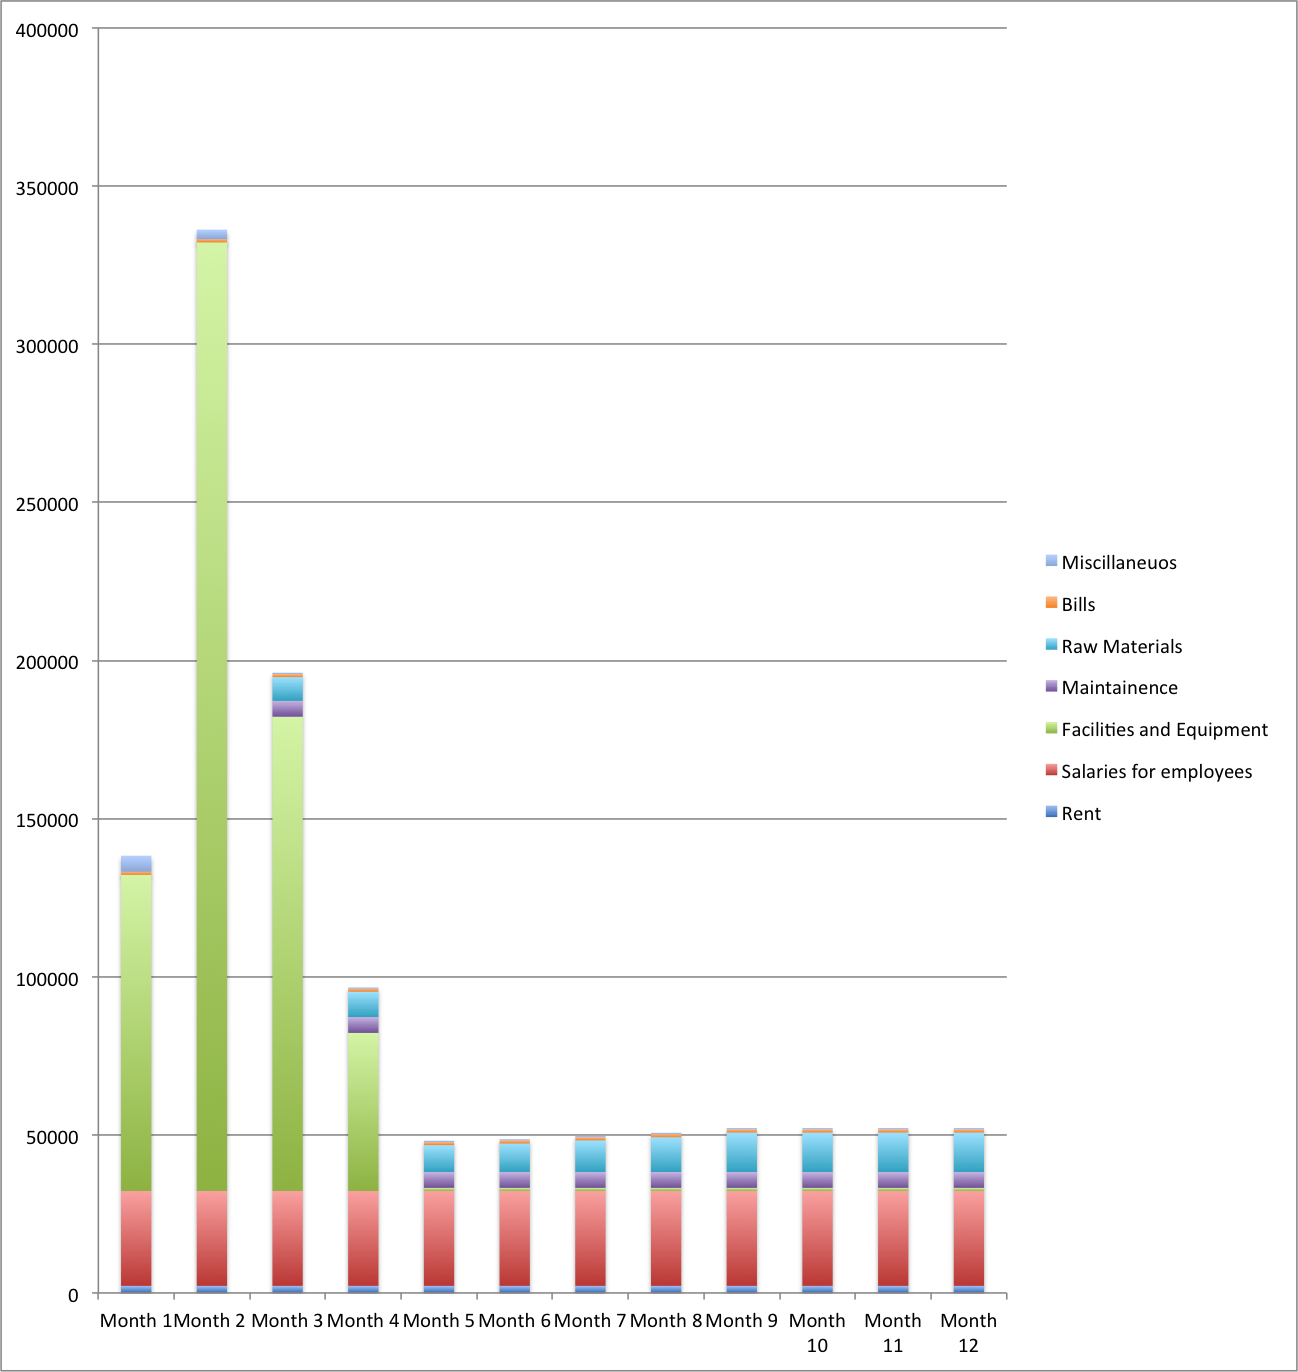
\includegraphics[width=\textwidth]{monthWiseCost.png}
	\end{figure}


      \subsubsection{Staff Hiring and Property}
We aim at setting up a microbrewery to start with in a manufacturing area in Himachal Pradesh \\
Rent in this area is roughly about Rs.1 / ft$^2$ per month. \\
As seen in the requirements: \\
There is a storage area required which has been estimated to: 500 sq $^2$. The area required of for manufacturing the product would be 3500 ft$^2$ this is plenty to space to meet estimated current requirements \\
Lunch area and office space is estimated to be about 1000 $^2$ as well this as above well allows some space for hiring a few more employees if and when needed. \\
Hence yearly rent works out at Rs. 60,000 per year. \\
The average cost of hiring for the skilled workers is about Rs. 1,00,000 a year we would require :
    \subsubsection{Staff Hiring and Property}
Since we aim at setting up a microbrewery to start with in at a manufacturing area in Himachal Pradesh

Rent in this area is roughly about Rs.1 / ft$^2$ per month.
As seen in the requirements:

there is a storage area required this has been estimated to: 500 sq $^2$ area of for manufacturing the product would be 1500 ft$^2$ this is plenty to space to meet estimated current requirements

    \begin{itemize}
\item 2 workers in charge of general processing as the business is small scale we will not need more
\item 1 worker in charge of general cleaning of the area
\end{itemize}

There will also be a security guard who will cost 50,000 a year
   \subsubsection{Ingredients}
cost of sugar -  Rs.30 / kg //
campden tables  - Rs.300 per 100 tablets //
Sweet mead Rs.500 for /128 gms //
//

This brings the cost of dry cider to Rs. 5.866 per 330 ml //
This brings the sweet of dry cider to Rs. 6.4 per 330 ml //

     \subsubsection{Equipment and Facilities}
     An entire list of equipment has been already been provided. Through use of websites and contacting a companies that do specialize in selling these products it has been estimated to cost about Rs. 6,00,000. This equipment will be ordered and paid for over a period of 3 months.//

The other expenses that have been listed as miscellaneous, products like stationary, furniture etc.

     %Funds needed for sales and marketing support

\newpage
%------------------------------------------------------------------------------%
%------------------------EXIT STRATEGY-----------------------------------------%
\section{Exit Strategy}
%Exit-trade sale

\newpage
%------------------------------------------------------------------------------%
%------------------------RISK ANALYSIS-----------------------------------------%
\section{Risk Analysis}

  \subsection{Risk Assessment and Management}
Identifying risks is mainly aimed at helping to outline a realistic budget requirement. Most of the items below are not avoidable, like staff illness or natural hazards. However some are, and foreseeing even the unavoidable ones can make them more manageable. Following is a comprehensive list of risks, including our approach to dealing with them.
   %Strong distribution channels minimise risk as does IP protection

  \begin{enumerate}
  \item Human related risks
    \begin{itemize}
    \item Delayed production \\ Whether it is because of suppliers delivering ingredients late or to do with the quality of the delivered product, we should have either a week's worth safety batch, which implies buying a freezer, or be prepared to deal with the cost of delayed production.
    \item Late distribution \\
The small scale of our business means space is limited which may cause a problem if buyers are late with picking up the merchandise. We should consider having an emergency courier  or again be prepared to deal with the const of delayed production.
    \item Experience of employees \\
Providing a training session is sometimes insufficient for ensuring perfect performance from our employees. We must be prepared to deal with the cost of flawed batches.
    \item Injuries, illness, misbehaviour \\
Anything that leads to an employee not being able to perform his tasks on a given day should be considered as a potential delay and extra cost.
    \end{itemize}

  \item Equipment related risks
    \begin{itemize}
    \item Break down \\
The extra cost that comes with machines breaking down can be reduced by a good warrantee on each piece of equipment, insurance and availability of spare parts.
    \item Power cut \\
Whilst inevitable, this risk can be counterbalanced if our contract with utilities providers includes compensations for this type of situation. We must also ensure our production can endure a long standby time and again be able to handle the cost of potentially loosing a batch.
    \item Water contamination \\
%not sure about this
The scale of our business does not permit a water filtering system which means we must test the quality of the provided water daily.
    \end{itemize}

  \item Ethical risks
    \begin{itemize}
    \item Working environment
    \item Religious employees
    \item Waste disposal \\
Waste disposal can be a sensitive issue with locals. Some of our waste may be have particularly unpleasant odour due to its biodegradable nature. We must try and find a way of donating apple residue to nearby farmers.
    \end{itemize}
  \end{enumerate}

\newpage
%------------------------------------------------------------------------------%
%------------------------COMPANY STRUCTURE AND MANAGEMENT PROFILES-------------%
\section{Company Structure and Management Profiles}

  \subsection{Current Equity Structure and Management}
  %Clear ownership structure
  Shimla Gold has been established an Indian Limited Company. The company is divided into 10,000 ordinary shares. Each share carries one vote per share, and is equally entitled in dividends.

  %Expirences management team

  We understand that is very important to have a clear decision structure from day one.
  The members of the team have to know which areas of the company they are responsible for.
  Therefore we have decided on the following management structure:
  \begin{itemize}
  \item Chief Executive Officer (CEO) - John Walker - long term strategy and planning
  \item Chief Operating Officer (COO) - Adam Fiksen - daily operations of the company, making sure that everything operates smoothly and according to the schedule
  \item Chief Financial Officer (CFO) - Rutwik Shah - financial records, risk and planning, monitoring and analysis of financial state of the company
  \item Chief Brand Officer (CBO) - Sahil Jain - brand image, marketing, advertisement and and public relations
  \item Chief Technical Officer (CTO) - Giovanni Charles - scientific and technological issues, research and improvements of the company
  \item Founders - Alina Boghiu, Lukasz Koprowski - helping in every day operations
  \end{itemize}

  COO, CFO, CBO and CTO report directly to the CEO, with CEO having the final vote in the case of any disagreement.
  Members of lower management are reporting to the COO.
  By giving the CEO power to have the last word, we are ensuring that in no case a disagreement will lead to a deadlock.
  We recognise that a deadlock an inability to quickly react may be a death sentence for a small company, and we want to avoid it at all cost.
  CEO should be able to make decisions and proceed with his plane.
  At the same time we support balance of power and recognise that no CEO should have absolute power and make arbitrary decisions for the entire company.
  A vote of owners should be able to remove the CEO if he is incapable or he lacks management skills.
  Therefore we have decided on the following division of initial shares:

  \begin{itemize}
  \item19\% - CEO - John Walker
  \item19\% - COO - Adam Fiksen
  \item14\% - CFO - Rutwik Shah
  \item14\% - CBO - Sahil Jain
  \item14\% - CTO - Giovanni Charles
  \item10\% - Alina Boghiu
  \item10\% - Lukasz Koprowski
  \end{itemize}

  To ensure commitment to the company and the level of effort relative to the level of shares we have decided on a four years vesting schedule.

  \subsection{The Team}
  
\includegraphics[width=80px]{john.jpg} \textbf{John Walker, Chief Executive Officer \& Co-Founder}\\
  John is the CEO an Co-Founder of Shimla Gold.
  He is a born leader and a pragmatist who translates a vision into a product.
  He is currently studying Computing at Imperial College London.

  Even when skydiving he is daydreaming about the future of the company.

  
\includegraphics[width=80px]{adam.jpg} \textbf{Adam Fiksen, Chief Operating Officer \& Co-Founder}\\
  Adam is a yet another student of Imperial College London.
  A skillful leader and manager.
  His experience in bar industry makes him a perfect hit for commanding day to day operations.

  When taking a break from the brewery, Adam raids elephants and looks forward to another crazy adventure.

  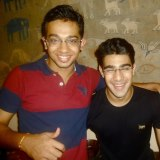
\includegraphics[width=80px]{rutwik.jpg} \textbf{Rutwik Shah, Chief Financial Officer \& Co-Founder}\\
  Rutwik is responsible for our accounting and finance.
  His deep insight into Indian law and economics makes him our tax ninja.
  He is also a Computing student at Imperial College London.

  When he is not stressing out about the state of our accounts he enjoys riding motorcycles.

  
\includegraphics[width=80px]{sahil.jpg} \textbf{Sahil Jain, Chief Brand Officer \& Co-Founder}\\
  Sahil is our insight into the Indian market.
  His understanding of culture and habits in invaluable to us.
  He oversees all our operations and advices on issues concerning our brand image.

  Even when he is not working on new marketing ideas, by playing golf he keeps building a valuable network of connections.

  
\includegraphics[width=80px]{gio.jpg} \textbf{Giovanni Charles, Chief Technical Officer \& Co-Founder}\\
  Giovanni is a Computing student at Imperial College London.
  In brewing, his passion for engineering translated into the love for detail and accuracy.
  He makes sure that our procedures follow the best standards and yield the best results.

  When he is not trying to come up with a new mind-blowing recipe or equipment he is busy producing DJ sets.

  
\includegraphics[width=80px]{alina.jpg} \textbf{Alina Boghiu, Black Ops \& Co-Founder}\\
  Alina is an Imperial College graduate.
  She works the super cool secret stuff.

  
\includegraphics[width=80px]{lukasz.jpg} \textbf{Lukasz Koprowski, Co-Founder}\\
  When not helping with production he pretends to know something about Programming.

\newpage
%------------------------------------------------------------------------------%
%------------------------ANNEX 1-----------------------------------------------%

\section{ANNEX 1 \\ Market Players}


\newpage

%------------------------------------------------------------------------------%
%------------------------ANNEX 2-----------------------------------------------%

\section{ANNEX 2} \\ Conclusion}
As a conclusion to our business proposition we would like to outline a few learning outcomes this experience has provided us with.\\

\noindent Firstly, being put in the situation of having to think about the implementation details of a business has shown us the benefits of being able to follow a well defined plan and the advantages of being organised as a team. Whilst the business idea might be fairly easy to explain, its implementation, however small the scale, raises an endless stream of problems to be solved and questions to be answered which prove both the capacity and the limitations of human intuition. For this reason it is extremely important to follow a rigorous plan and try to foresee as many risks as possible, as it is impossible to control the flow of events completely. \\

\noindent Secondly, we learnt there is much more to selling a product than making it available. Whilst a good product will advertise itself, it is important to sell the entire experience that goes with it and be prepared for both expansion or having to start over from scratch. Looking at success and failure stories of other startups whilst trying to outline the plan for our own business development, we saw that luck, whilst helpful, is replaceable with careful financial estimations, a pessimistic timeline and clever safety measures. \\

\noindent Finally, we saw that in order to make good use of resources and come across as reliable the leading team must have well defined roles, in accordance with their skills. in order for potential investors to trust we can accomplish our goals, it is important to have a constant sense check when planning development and remain realistic.\\

\noindent We consider this exercise to have been a worthwhile experience for having shown us a more comprehensive way of thinking about projects in general.

\newpage
%------------------------------------------------------------------------------%
%------------------------ANNEX 3-----------------------------------------------%

\section{ANNEX 3 \\ Company Background}
Shimla Gold Cider is the vision of 7 computing students from Imperial College London, we've all been good friends for a long time and last summer Giovanni and Adam went to visit Rutwik and Sahil in India, during their time there they made a peculiar observation that they couldn't find any cider in India. \\

\noindent They asked Sahil and Rutwik about this and they couldn't provide an explanation even in the areas of India frequented by cider accustomed westerners such as Goa, there was just no cider. At first we thought maybe the taste just didn't agree with the Indian culture but we know first hand that many of our Indian friends enjoy it when abroad, it just seemed that nobody had introduced it yet. \\

\noindent It was from this simple observation the idea to bring cider to the Indian market was conceived. Shimla is the area of India where apples were first introduced by Samuel Evan Stokes and remains the heart of apple cultivation today. Shimla was regarded and the capital of Summer time India by the British which we believe nicely reflects the Anglo-Indian dynamic of our team, we hope to add to the historic reputation of Shimla by making it the birth place of Shimla Gold Cider.

\newpage
%------------------------------------------------------------------------------%
%------------------------------------------------------------------------------%
\section{ANNEX 4}

\begin{figure}[h!]
	\caption{First Year Costs and Financial Projections}
	\centering
	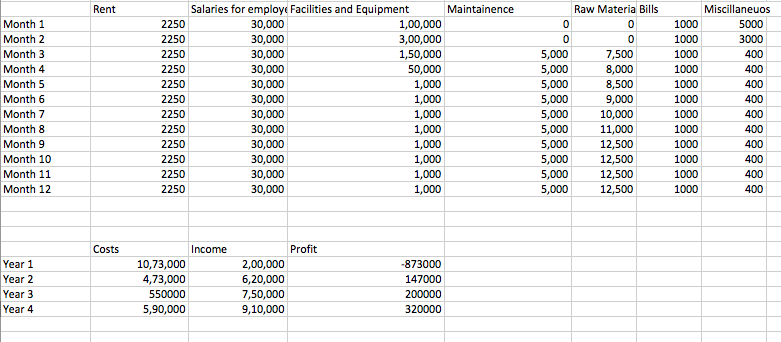
\includegraphics[width=\textwidth]{costs.png}
\end{figure}
\newpage
%------------------------------------------------------------------------------%
%------------------------------------------------------------------------------%
\end{document}
